\section{Limits on New Physics}
\label{sec:limit}

As discussed in Sec.~\ref{sec:results}, we do not observe any excess in the signal regions.
We use these results to place Bayesian95\% confidence level upper limits~\ref{cl95cms} on 
the non-SM contributions to the yields in the signal regions, using a log-normal model
of nuissance parameter integration. The results are summarized in Table~\ref{resultsyieldtable}.  


\begin{figure}[hbt]
\begin{center}
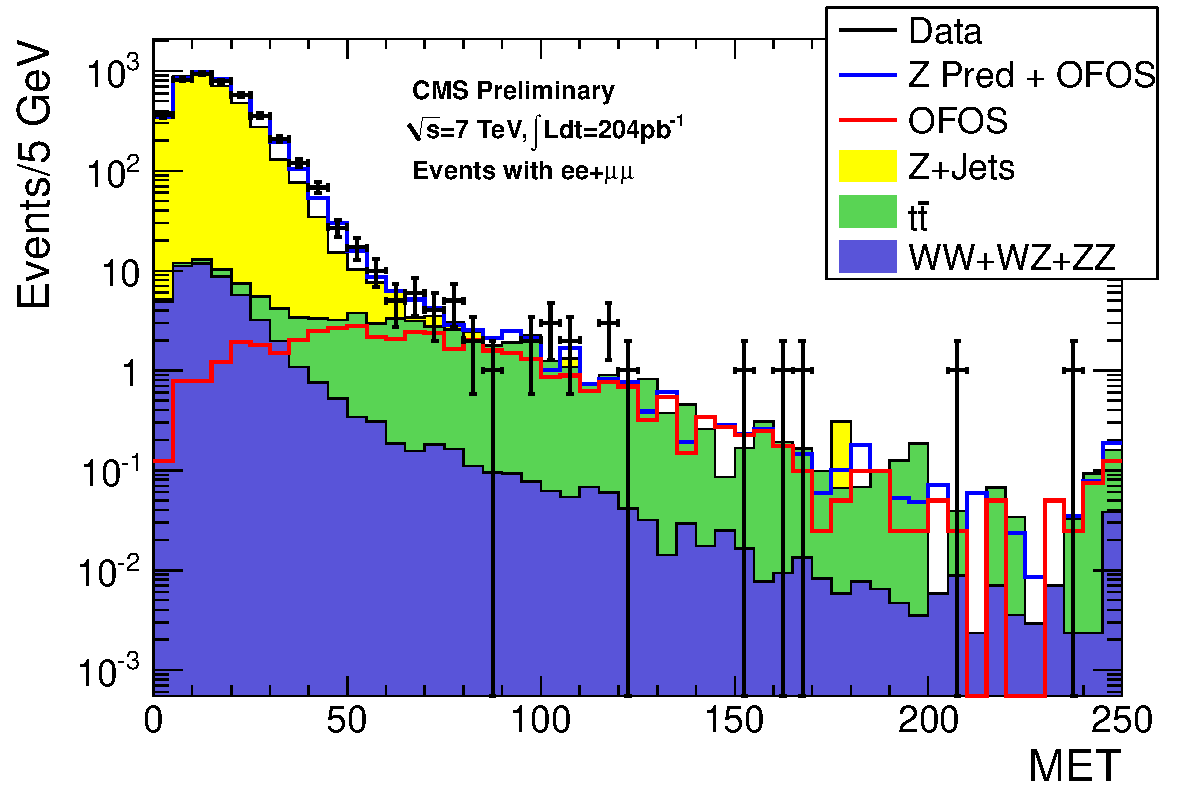
\includegraphics[width=0.78\linewidth]{plots/lep_metPredicted.pdf}
\caption{\label{fig:results}\protect 
     The observed MET distribution for data in the (black points),
      predicted $t\bar{t}$ MET distribution (red line), the sum of predicted %
	  $t\bar{t}$ MET distribution ad
      Z  MET  distribution  predicted  from photon  MET  templates
      (solid blue line),  and MC stacked for dominant backgrounds. 
	  %Here $VV$  indicates the sum
      %of  $WW$,  $WZ$  and  $ZZ$, while  additional  backgrounds  from
      %$W+$jets   and   single  top   are   omitted   since  they   are
      %negligible.  
}
\end{center}
\end{figure}

\begin{table}[htb]
\begin{center}
\caption{\label{resultsyieldtable} 
Summary of the yields in the regions MET $>$ 30, 60, 100 and 200 GeV. The total predicted yield is the sum of the
predicted background from \Z plus jets from the MET templates method (\Z pred) plus the \ttbar\ contribution
predicted from OF subtraction. The 95\% CL Bayesian UL is indicated, as well as the expected NLO yields for the
LM4 and LM8 scenarios.
{\bf UPDATE TABLE}
}
    \begin{tabular}{lcccc}
\hline
                        &   N(MET $>30$)  GeV    &   N(MET $>60$)  GeV    &   N(MET $>100$) GeV    &   N(MET $>200$) GeV \\
\hline
      $Z$ pred    &  406.54  $\pm$  6.82  &   14.63  $\pm$  1.27  &    1.82  $\pm$  0.60  &    0.19  $\pm$  0.07 \\
 OF subtraction   &   54.77  $\pm$  2.09  &   34.73  $\pm$  1.67  &   11.76  $\pm$  0.97  &    1.13  $\pm$  0.33 \\
\hline
 total predicted  &  461.31  $\pm$  7.13  &   49.36  $\pm$  2.10  &   13.59  $\pm$  1.14  &    1.32  $\pm$  0.34 \\
\hline
      observed    &                  488  &                   39  &                   14  &                    2 \\
\hline
            UL    &                    X  &                   39  &                   14  &                    2 \\
\hline
           LM4    &                    X  &                   39  &                   14  &                    2 \\
           LM8    &                    X  &                   39  &                   14  &                    2 \\
\hline
\end{tabular}
\end{center}
\end{table}

